\lab{Principal Component Analysis and Latent Semantic Indexing}{PCA and LSI}
\objective{Understand the basics of principal component analysis and latent semantic indexing.}
\label{lab:pca}

\section*{Principal Component Analysis}
Understanding the variance in complex data is one of the initial tasks in exploratory data analysis. For example, consider the scatter plot  displaying the sepal and petal lengths of 100 different irises shown in Figure \ref{fig:iris_1}.
\begin{figure}
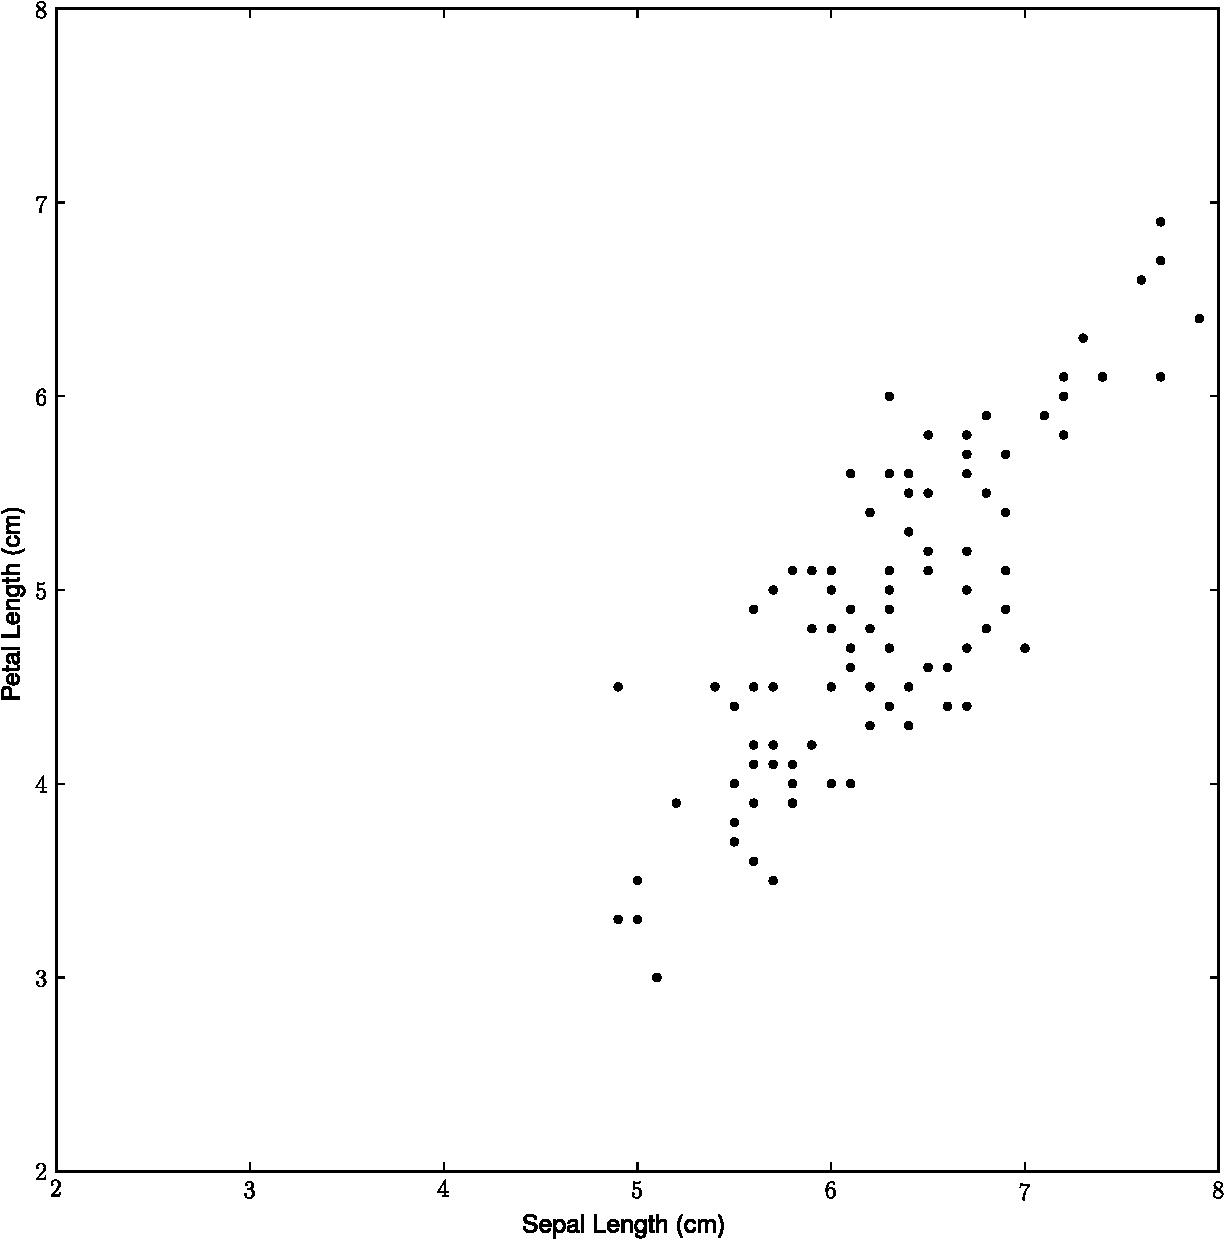
\includegraphics[width=\textwidth]{iris0.pdf}
\caption{Sepal Length vs. Petal Length for 100 iris flowers. Note the strong correlation of these variables.}
\label{fig:iris_1}
\end{figure}
There are three distinct types of iris flowers present: \emph{setosa}, \emph{versicolor}, and \emph{virginica}.
Considering this data, we might ask how to best distinguish the different types of irises given the data about their sepal and petal lengths.
We can answer this question by finding the characteristic that causes the greatest variance in the data.
(Greater variance implies a greater ability to distinguish between data points. If the variance is very small, the data are clustered tightly together, and it is difficult to distinguish well.)

Upon examination, we see that the petal length ranges between $3$ and $7$ cm, while the sepal length only ranges between $5$ and $8$ cm. We might be tempted to say that the most distinguishing aspect of irises is their petal length, but this is only considering the features of the data individually, and not collectively. The two features of the data are clearly correlated, and a more careful consideration would lead us to conclude that the most distinguishing aspect of irises is their overall size. Some irises are are much bigger than others while the sepal and petal lengths stay roughly in proportion.
\begin{figure}
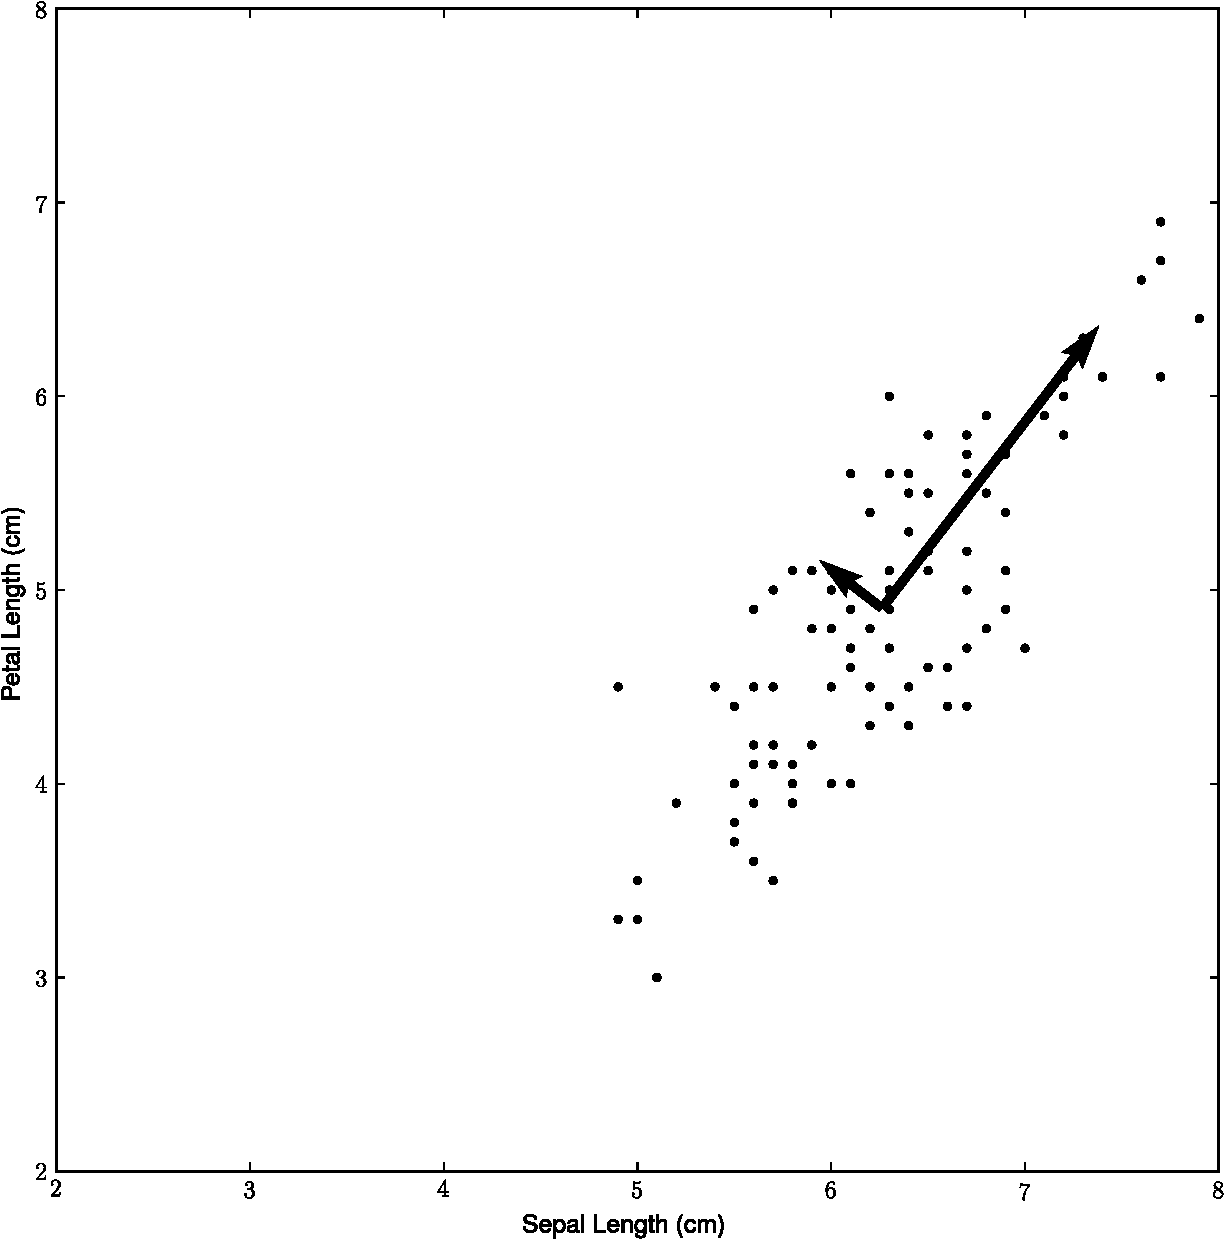
\includegraphics[width=\textwidth]{iris2.pdf}
\caption{The vectors indicate the two principal components weighted by their contribution to the variance.}
\label{fig:iris_2}
\end{figure}

Principal Component Analysis (PCA) is a multivariate statistical tool used to orthogonally change the basis of a set of observations from the basis of original features (which may be correlated) into a basis of uncorrelated (in fact, orthonormal) variables called the \emph{principal components}. It is a direct application of the singular value decomposition (SVD) from linear algebra. More specifically, the first principal component will account for the greatest variance in the set of observations, the second principal component will be orthogonal to the first, accounting for the second greatest variance in the set of observations, etc. The first several principal components capture most of the variance in the observation set, and hence provide a great deal of information about the data. By projecting the observations onto the space spanned by the principal components, we can reduce the dimensionality of the data in a manner that preserves most of the variance.

In our iris example, the two principal components are shown in Figure \ref{fig:iris_2}. The first principal component, corresponding intuitively to iris size, accounts for $96\%$ and of the variance in the data. The second, which accounts for only $4\%$ of the variance, corresponds to the relative sepal and petal length in irises of the same size.

\subsection*{Computing the Principal Components}
We now explore how to use the SVD to compute the principal components of a data set.
Throughout we will use the iris data set, which can be obtained as follows:
\begin{lstlisting}
>>> import numpy as np
>>> from scipy import linalg as la
>>> import sklearn.datasets as datasets
>>> iris = datasets.load_iris()
>>> X = iris.data
\end{lstlisting}
We represent the collection of observations as a matrix $n \times m$ matrix $X$, where each row of $X$ is an observation, and each column is a specific feature.
Let $k = \min(m,n)$.
In the iris example, $X$ contains 150 observations, each consisting of 4 features, as shown below:
\begin{lstlisting}
>>> X.shape
(150L, 4L)
>>> iris.feature_names
['sepal length (cm)',
 'sepal width (cm)',
 'petal length (cm)',
 'petal width (cm)']
\end{lstlisting}

The first step in PCA is to pre-process the data. In particular, we first translate the columns of $X$ to have mean 0.
The data may then be optionally scaled to remove discrepancies arising from different units of measure (i.e. centimeters vs meters), and we call the centered and scaled data $Y$.
In this lab, we will not have any scaling issues, so we won't address this further.
We pre-process our iris data as follows:
\begin{lstlisting}
>>> Y = X - X.mean(axis=0)
\end{lstlisting}

We next compute the truncated SVD of our centered and scaled data,
\[Y = U\Sigma V^{T}\]
where $U$ is $n \times k$, $\Sigma$ is a $k\times k$ diagonal matrix containing the singular values of $Y$ in decreasing order along the diagonal, and $V$ is $m \times k$. The columns of $V$ are the principal components (which form an orthonormal basis for the space spanned by the observations), and the corresponding singular values provide us information about how much variance is captured in each principal component. More specifically, let $\sigma_{i}$ be the $i$-th non-zero singular value. Then the value
\[\frac{\sigma^2_{i}}{\sum_{j=1}^{k} \sigma^2_{j}}\]
is the percentage of the variance captured by the $i$-th principal component.
We compute the truncated SVD of the iris data and show the variance percentages for each component below:
\begin{lstlisting}
>>> U,S,VT = la.svd(Y, full_matrices=False)
>>> S**2/(S**2).sum() # variance percentages
array([ 0.92461621,  0.05301557,  0.01718514,  0.00518309])
\end{lstlisting}

In general, we are only interested with the first several principal components. How many principal components exactly should we keep? There are a number of ways to decide this. One is to only keep the first two principal components, as these enable us to project the data into $2$-dimensional space, which is easy to visualize. Another way is to only keep the set of principal components accounting for a certain percentage (say $80\%$) of the variance. A third method is to examine the \emph{scree plot} of the variance percentages for each principal component, as in Figure \ref{fig:iris_scree}.
\begin{figure}
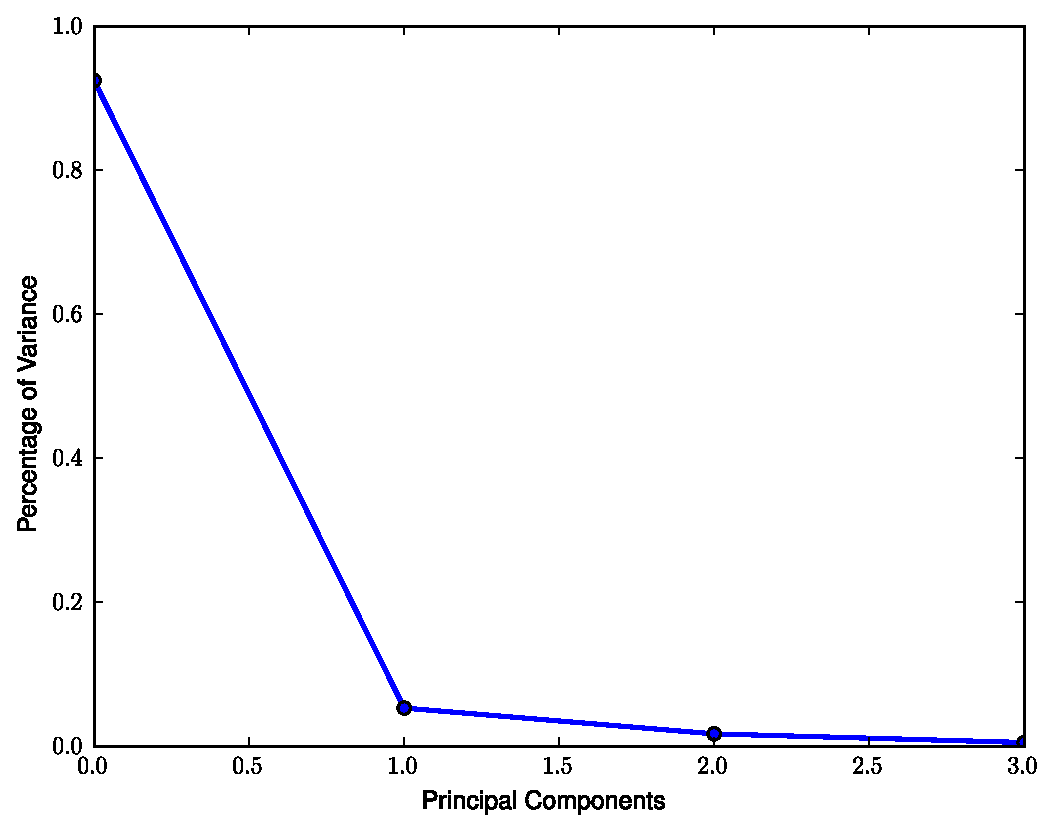
\includegraphics[width=\textwidth]{iris_scree.pdf}
\caption{Scree plot of the percentage of variance for PCA on the iris dataset.}
\label{fig:iris_scree}
\end{figure}
Upon examination of the iris scree plot, we see that there is a distinct change after the first principal component. This method is referred to as finding the ``elbow" of the scree plot, and we keep all the principal components on the left of the elbow. In the case of the iris data, that is simply the first principal component, which accounts for $92\%$ of the variance.

Once we have decided how many principal components to keep (say the first $l$), we can project the observations from the original feature space onto the principal component space by computing
\begin{equation*}
\widehat{Y} = U_l\Sigma_l
\end{equation*}
where $\Sigma_l$ is the first $l$ rows of $\Sigma$ and $U_l$ is the first $l$ columns of $U$.
Using the SVD formula, note that
\[
\widehat{Y} = YV_l,
\]
where $V_l$ is the first $l$ columns of $V$.
In this way, we see that the $i$-th row of $\widehat{Y}$ is simply the projection of the $i$-th observation onto the orthonormal set of the first $l$ principal components.
Under this projection, the data is represented in fewer dimensions, and in such a way that accentuates the variance (which can help with finding patterns within the data).

In Figure \ref{fig:iris_pca} we display the transformed iris data set, plotting the first principal component against the second. This reduction helps us to see the distinctions between the three different species, using only two dimensions instead of the full four dimensions of the feature space.
\begin{figure}
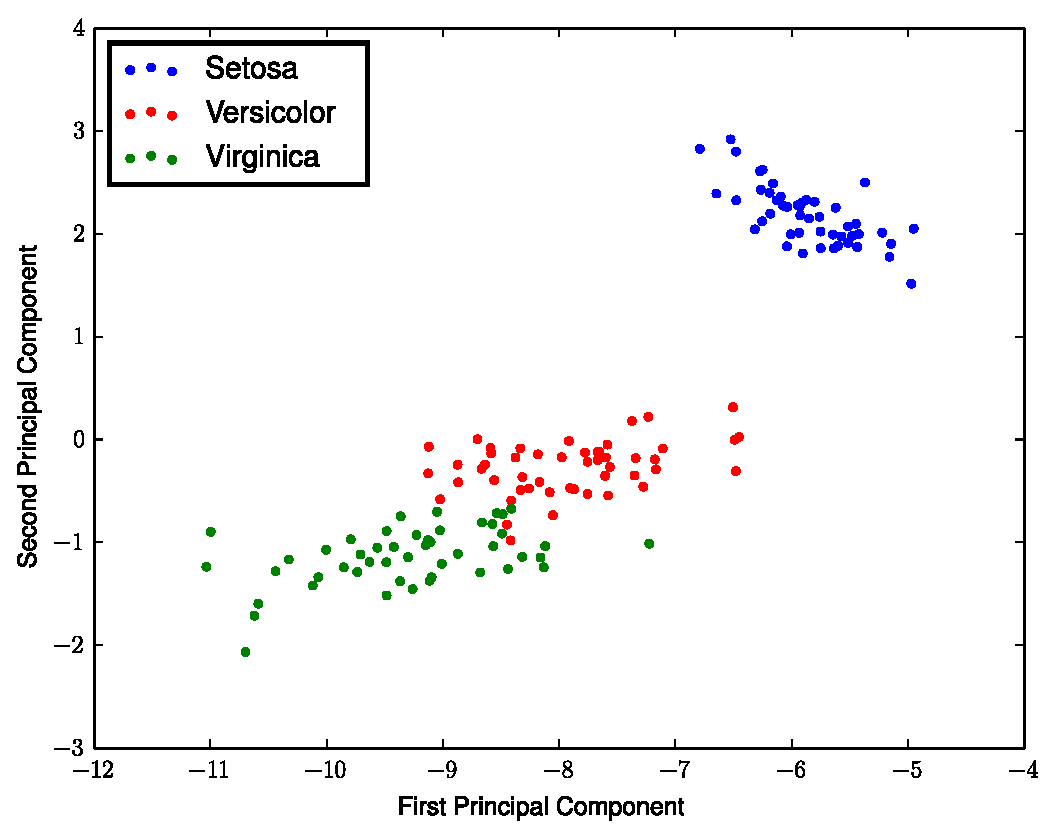
\includegraphics[width=\textwidth]{iris_pca.pdf}
\caption{Plot of transformed iris data, keeping only the first two principal components.}
\label{fig:iris_pca}
\end{figure}

\begin{problem}
Recreate the plot shown in Figure \ref{fig:iris_pca} by performing PCA on the iris dataset, keeping the first two principal components.

\emph{Note:}
If \li{Yhat} is your $150 \times 2$ array of transformed observations, you can access the rows corresponding to the setosa flowers as follows:
\begin{lstlisting}
>>> Yhat[iris.target==0]
\end{lstlisting}
To get the rows corresponding to versicolor and virginica specimens, simply replace the $0$ with $1$ and $2$, respectively.
\end{problem}

\section*{Latent Semantic Indexing}
\emph{Latent Semantic Indexing} (LSI) is an application of the ideas of PCA to the realm of natural language processing.
In particular, LSI employs the SVD to reduce the dimensionality of a large corpus of text documents and to enable us to evaluate the similarity between two documents.
Many information retrieval systems used in government and industry are based on LSI.

To motivate the problem, suppose we have a large collection of documents dealing with various statistical and mathematical topics.
How can we find an article about PCA?
We might consider simply choosing the article that contains the acronym \emph{PCA} the greatest number of times, but this is a crude method.
A better way is to use a form of PCA on the collection of the documents.

In order to do so, we need to represent the documents as numerical vectors.
A standard way of doing this is to define an ordered set of words occurring in the collection of documents (called the \emph{vocabulary}), and then
represent each document as a vector of word counts from the vocabulary.
More formally, let our vocabulary be $V = \{w_1,w_2,\ldots,w_m\}$.
Then a document is a vector $x  = (x_1,x_2,\ldots,x_m) \in \mathbb{R}^m$ such that $x_i$ is the number of occurrences of word $w_i$ in the document.
In this setup, we represent the entire collection of $m$ documents as an $n \times m$ matrix $X$, where $m$ is the length of the vocabulary and $n$ is the number of documents in our collection, each row being a document vector.
As expected, we let $X_{i,j}$ be the number of times term $j$ occurs in document $i$.
Note that $X$ is often a sparse matrix, as any one document likely doesn't contain most of the vocabulary words.
This mode of representation is called the \emph{bag of words} model for documents.

We calculate the SVD of $X$ without centering or scaling the data so that we may retain the sparsity.
We now have $X = U\Sigma V^T$. Once we have selected the number of principal components to keep, say $l$, we can represent the corpus of documents by the matrix
\[
\widehat{X} = U_l\Sigma_l.
\]
Note that $\widehat{X}$ will no longer be a sparse matrix, but it has dimensions $n \times l$, which is much smaller than $n \times m$ when $l \ll m$.

Now that we have our documents represented in terms of the first $l$ principal components, we can find the similarity between two documents.
Our measure for similarity is just the cosine of the angle between the vectors; a small angle (and hence large cosine) indicates greater similarity, while a large angle (hence small cosine)
indicates greater dissimilarity.
Recall that we can use the inner product to find the cosine of the angle between two vectors.
Under this metric, the similarity between document $i$ and document $j$ (represented by the $i$-th and $j$-th row of $\widehat{X}$, notated $\widehat{X}_i$ and $\widehat{X}_j$, respectively) is just
\[
\frac{\langle \widehat{X}_i, \widehat{X}_j\rangle}{\|\widehat{X}_i\|\|\widehat{X}_j\|}.
\]
To find the document most similar to document $i$, we simply compute
\[
\argmax_{j\neq i} \frac{\langle \widehat{X}_i, \widehat{X}_j\rangle}{\|\widehat{X}_i\|\|\widehat{X}_j\|}.
\]


We now discuss some practical issues involved in creating the bag of words representation $X$ from the raw text.
Our data set will consist of the US State of the Union addresses from 1945 through 2013, each contained in a separate text file in the folder {\tt Addresses}.
We would like to avoid loading in all of the text into memory at once, and so we will \emph{stream} the documents one at a time.

The first thing we need to establish is the vocabulary set, i.e. the set of unique words that occur throughout the collection of documents.
A Python set object automatically preserves the uniqueness of the elements, so we will create a set, and then iteratively read through the documents, adding the unique words of each
document to the set. As we read in each document, we will remove punctuation and numerical characters and convert everything to lower case.
The following code will accomplish this task:
\begin{lstlisting}
>>> # get list of filepaths to each text file in the folder
>>> import string
>>> from os import listdir
>>> path_to_addresses = "./Addresses/"
>>> paths = [path_to_addresses + p for p in os.listdir(path_to_addresses) if p[-4:]==".txt"]

>>> # helper function to get list of words in a string
>>> def extractWords(text):
>>>     trans = string.maketrans("", "")
>>>     return text.strip().translate(trans, string.punctuation+string.digits).lower().split()

>>> # initialize vocab set, then read each file and add to the vocab set
>>> vocab = set()
>>> for p in paths:
>>>     with open(p, 'r') as f:
>>>         for line in f:
>>>             vocab.update(extractWords(line))
\end{lstlisting}

We now have a set of all the unique words in the corpus. However, many of the most common words do not provide important information.
We call these \emph{stop words}. Examples in English include \emph{the, a, an, and, I, we, you, it, there}, etc;
a list of common English stop words is given in {\tt stopwords.txt}.
We remove the stopwords from our vocabulary set as follows, and then fix an ordering to the vocabulary by creating a dictionary
whose key-value pairs are of the form (word, index):
\begin{lstlisting}
>>> # load stopwords
>>> with open("stopwords.txt", 'r') as f:
>>>     stopwords = set([w.strip().lower() for w in f.readlines()])

>>> # remove stopwords from vocabulary, create ordering
>>> vocab = {w:i for i, w in enumerate(vocab.difference(stopwords))}
\end{lstlisting}

We are now ready to create the word count vectors for each document, and store these in a sparse matrix $X$.
It is convenient to use the \li{Counter} object from the \li{collections} module, as this
object automatically counts the occurrences of each distinct element in a list.
\begin{lstlisting}
>>> from scipy import sparse
>>> from collections import Counter
>>> counts = [] # holds the entries of X
>>> doc_index = [] # holds the row index of X
>>> word_index = [] # holds the column index of X

>>> # iterate through the documents
>>> for doc, p in enumerate(paths):
>>>     with open(p, 'r') as f:
>>>         # create the word counter
>>>         ctr = Counter()
>>>         for line in f:
>>>             ctr.update(extractWords(line))
>>>         # iterate through the word counter, store counts
>>>         for word, count in ctr.iteritems():
>>>             try: # only look at words in vocab
>>>                 word_index.append(vocab[word])
>>>                 counts.append(count)
>>>                 doc_index.append(doc)
>>>             except KeyError: # if word isn't in vocab, skip it
>>>                 pass

>>> # create sparse matrix holding these word counts
>>> X = sparse.csr_matrix((counts, [doc_index,word_index]), shape=(len(paths),len(vocab)), dtype=np.float)
\end{lstlisting}

\begin{problem}
Using the techniques of LSI discussed above applied to the word count matrix $X$ and keeping the first 7 principal components,
find the most similar and least similar speeches to Bill Clinton's 1993 speech and Richard Nixon's 1974 speech.
Are the results plausible?

\emph{Hint:} Since $X$ is a sparse matrix, you will need to use the SVD method found in \li{scipy.sparse.linalg}.
This method operates slightly differently than the SVD method found in \li{scipy.linalg}, so make sure to read the
documentation.
\label{prob:LSI1}
\end{problem}

The simple bag of words representation is a bit crude, as it fails to consider how some words may be more important than others
in determining the similarity of documents.
Words appearing in few documents tend
to provide more information than words occurring in every document.
For example, while the word \emph{war} might not be considered a stop word,
it is likely to appear in quite a few addresses, whereas \emph{Afghanistan} will not.
Thus two speeches sharing the word \emph{Afghanistan} ought to be considered more
related than two speeches sharing the word \emph{war}.
So while $X_{i,j}$ is a good measure of the importance of term $j$ in document $i$,
we also need to consider some kind of global weight for each term $j$,
indicating how important the term is over the entire collection.
There are a number of different weights we could choose; we choose to employ
the following approach.

Let $t_{j}$ be the total number of times term $j$ appears in the entire
collection of documents.
Define
\begin{equation*}
p_{i,j} = \frac{X_{i,j}}{t_{j}}.
\end{equation*}
We then let
\begin{equation*}
g_{j} = 1 + \sum_{i=1}^{m} \frac{p_{i,j} \log (p_{i,j} + 1)}{\log m},
\end{equation*}
where $m$ is the number of documents in the collection.
We call $g_{j}$ the \emph{global weight} of term $i$.
We replace each term frequency in the matrix $X$ by weighting it globally.
Specifically, we define a matrix $A$ with entries
\begin{equation*}
A_{i,j} = g_{j} \log (X_{i,j} + 1).
\end{equation*}
We can now perform LSI on the matrix $A$, whose entries are both locally and globally weighted.

To calculate the matrix $A$ in a streaming manner, we must alter our code above somewhat:
\begin{lstlisting}
>>> from itertools import izip
>>> from math import log
>>> t = np.zeros(len(vocab))
>>> counts = []
>>> doc_index = []
>>> word_index = []

>>> # get doc-term counts and global term counts
>>> for doc, path in enumerate(paths):
>>>     with open(path, 'r') as f:
>>>         # create the word counter
>>>         ctr = Counter()
>>>         for line in f:
>>>             words = extractWords(line)
>>>             ctr.update(words)
>>>         # iterate through the word counter, store counts
>>>         for word, count in ctr.iteritems():
>>>             try: # only look at words in vocab
>>>                 word_ind = vocab[word]
>>>                 word_index.append(word_ind)
>>>                 counts.append(count)
>>>                 doc_index.append(doc)
>>>                 t[word_ind] += count
>>>             except KeyError:
>>>                 pass

>>> # get global weights
>>> g = np.ones(len(vocab))
>>> logM = log(len(paths))
>>> for count, word in izip(counts, word_index):
>>>     p = count/float(t[word])
>>>     g[word] += p*log(p+1)/logM

>>> # get globally weighted counts
>>> gwcounts = []
>>> for count, word in izip(counts, word_index):
>>>     gwcounts.append(g[word]*log(count+1))

>>> # create sparse matrix holding these globally weighted word counts
>>> A = sparse.csr_matrix((gwcounts, [doc_index,word_index]), shape=(len(paths),len(vocab)), dtype=np.float)
\end{lstlisting}

\begin{problem}
Repeat Problem \ref{prob:LSI1} using the matrix $A$. Do your answers seem more reasonable than before?
\end{problem}
